\documentclass[11pt,a4paper]{article}

\usepackage[margin=2cm]{geometry}
\usepackage{amsmath,amssymb}
\usepackage{booktabs}
\usepackage{graphicx}
\usepackage{microtype}
\usepackage{setspace}
\usepackage{parskip}
\usepackage{abstract}
\usepackage{tabularx}
\usepackage{xcolor}
\usepackage{xspace}
\usepackage[hidelinks]{hyperref}

\newcommand{\model}{\texttt{Qwen3-4B-Instruct-2507}\xspace}
\newcommand{\code}[1]{\nolinkurl{#1}}
\newcommand{\prompt}[1]{\texttt{#1}}
% Recalculate after all textual and figure revisions are complete.
\newcommand{\reportwordcount}{4,917}

\begin{document}
\onehalfspacing
\pagenumbering{roman}

\begin{titlepage}
    \centering
    \vspace*{2.0cm}
    {\LARGE\bfseries Tracing Small Circuits in an Open Language Model\par}
    \vspace{0.5cm}
    {\Large A Reproducibility Study of Attribution Graphs in Qwen3-4B-Instruct\par}
    \vspace{2.0cm}
    {\large MPhil in Data Intensive Science\par}
    \vspace{0.5cm}
    {\large Project 28: Mechanistic Interpretability of Open Source LLMs\par}
    \vfill
    \begin{tabular}{ll}
        Candidate: & Evelyn Paskhaver \\
        Supervisor: & Miles Cranmer \\
        Date: & July 12, 2026 \\
        Word count: & \textbf{\reportwordcount} \\
    \end{tabular}
    \vfill
    % Verify the candidate details, word count and required declaration before submission.
\end{titlepage}
\clearpage
\pagenumbering{arabic}

\begin{abstract}
Anthropic's \emph{On the Biology of a Large Language Model} uses sparse features,
attribution graphs and causal interventions to formulate hypotheses about
mechanisms underlying language-model behaviour. The present study evaluates the
transferability of that methodology to the open-weight, 4-billion-parameter
\model. Two behaviours were
studied: addition, focusing on propagation of a carry between decimal columns,
and factual recall, instantiated by SI-unit and capital-city prompts. An
independent pipeline generated synthetic prompt sets, captured final-position MLP
outputs at seven layers, trained one 8,192-latent sparse autoencoder (SAE) per
layer, constructed gradient-based contrast attribution graphs, and performed
feature inhibition, latent swaps, raw-activation patches and component
knockouts.

The results provided partial support for methodological transfer. The clearest
factual-recall effect was a full-latent
force-to-energy patch: on the energy prompt, the probability of the force prefix
\texttt{new} rose from 0.0240 to 0.4980 and became the top prediction, while the
energy prefix \texttt{j} fell from 0.7969 to 0.2354. Graph-selected sparse swaps
were much weaker. In arithmetic, progressively ablating 73 graph-positive
features reduced the correct-minus-dropped-carry logit gap only from 7.12 to
6.63. A stronger full-latent patch reduced it to 0.74, whereas a raw MLP patch
transferred the source answer digit completely. A control source whose answer
digit was 2 transferred 2 rather than a generic no-carry state, indicating that
the intervention did not isolate carry as an independent variable. Capital-city
swaps remained weak even for high-confidence prompts.

The experimental workflow was therefore reproduced, and causal structure was
identified at the level of broad activations, but no Anthropic-like compact
sparse circuit was recovered. Several methodological factors plausibly account
for this discrepancy: the present SAEs were independently trained on only 800
final-position vectors per layer, their unconstrained $\ell_1$ objective has a scale
degeneracy, and several all-position interventions applied them outside their
training distribution. The findings consequently identify which components of
circuit tracing transferred under a lightweight open-model implementation and
which did not.
\end{abstract}

\clearpage
\tableofcontents
\clearpage

\section{Introduction}

Large language models can produce correct answers without exposing the internal
computations that produced them. Mechanistic interpretability attempts to replace
a purely input--output description with a causal account in terms of internal
representations and interactions. This is difficult because a model neuron need
not correspond to one human-understandable concept: multiple features may be
represented in superposition, making individual neurons polysemantic
\cite{elhage2022superposition}. Sparse autoencoders offer one possible change of
basis. They reconstruct an activation with a relatively small set of active
learned directions, which can sometimes be more interpretable and causally useful
than the original neurons \cite{cunningham2023sae,bricken2023monosemanticity}.

Lindsey et al. applied this general programme at much greater scale in
\emph{On the Biology of a Large Language Model} \cite{lindsey2025biology}. Their
case studies use attribution graphs to propose computational pathways for
behaviours including addition and factual recall, then test those pathways with
interventions. The companion methods work is explicit that a graph describes a
local replacement model and is a source of hypotheses, not automatically a
faithful explanation of the underlying model \cite{ameisen2025circuit}. This
qualification makes the work well suited to a reproducibility study: successful
reproduction requires both a plausible graph and the predicted causal effects in
the original model.

The present study evaluates that transfer in \model, an open-weight causal
language model with 4.0 billion parameters, 36 transformer layers and hidden
width 2,560 \cite{yang2025qwen3,qwenmodelcard}. The experimental design uses
small synthetic prompt corpora, independently trained SAEs at selected layers, a
pruned attribution-style graph, and causal validation by inhibition and
activation swapping. It thus evaluates the methodological sequence at a
substantially smaller scale than Anthropic's study rather than attempting an
architectural replication of the cross-layer transcoder. Addition and factual
recall constitute the two principal behaviours. Factual recall is evaluated in
two domains: capital cities, which parallel the target study's factual-recall
examples, and SI units, which provide a science-focused extension. The SI-unit
domain also permits controlled minimal pairs in which, for example,
\texttt{force} is replaced by \texttt{energy} while the remainder of the prompt
is held constant.

The investigation asks three questions:

\begin{enumerate}
    \item Can a lightweight, per-layer SAE pipeline identify sparse feature sets
    whose interventions predictably alter the model's output distribution?
    \item When sparse feature interventions are insufficient, is causal structure
    detectable at broader levels of the activation representation?
    \item Which methodological differences explain agreement or disagreement
    with the Anthropic result?
\end{enumerate}

Reproduction was assessed against criteria stricter than the observation of an
arbitrary logit change. The clean model was required to express the behaviour;
a graph-derived intervention was then required to move a pre-specified
target-versus-contrast quantity in the predicted direction; and the effect was
required to exceed changes attributable to numerical precision and, where
possible, to survive a reverse-direction or alternative-source control. Under
these criteria, the evidence supports a partial reproduction. Broad latent and
raw-activation patches demonstrate causal information, whereas sparse graph
features rarely control the predicted answer. The analysis therefore examines
why reconstruction quality, sparse attribution and mechanistic faithfulness
diverge in the present implementation.

\section{Background and relation to the target study}

\subsection{Sparse decompositions}

Let $x\in\mathbb{R}^{d}$ be an activation from a transformer component. A
one-hidden-layer SAE encodes $x$ into an overcomplete latent vector $z\in
\mathbb{R}^{m}$ and reconstructs it as $\hat{x}$:
\begin{align}
    z &= \operatorname{ReLU}\!\left(W_{\mathrm e}(x-b_{\mathrm d})+b_{\mathrm e}\right), \\
    \hat{x} &= W_{\mathrm d}z+b_{\mathrm d}.
\end{align}
When $m>d$, sparsity rather than dimensional compression is intended to make the
representation useful. If only a few coordinates of $z$ are non-zero for each example,
the decoder columns can be treated as candidate feature directions. Previous
work has shown that such decompositions can yield more interpretable units and
support causal edits in some settings \cite{cunningham2023sae,bricken2023monosemanticity}.
Neither low reconstruction error nor an overcomplete dictionary alone, however,
establishes that a latent is monosemantic or causally complete.

\subsection{Anthropic's attribution graphs}

The target study did not use independent per-layer SAEs as direct substitutes
for its model's computation. It used a 30-million-feature cross-layer transcoder
(CLT) for Claude 3.5 Haiku \cite{lindsey2025biology}. A feature at layer $\ell$
reads the residual stream at that layer and has separate decoder contributions
to the MLP outputs of layer $\ell$ and later layers. In simplified notation,
\begin{align}
    a^{\ell} &= \operatorname{JumpReLU}(W_{\mathrm{enc}}^{\ell}x^{\ell}), \\
    \hat{y}^{\ell} &= \sum_{k\leq \ell}W_{\mathrm{dec}}^{k\rightarrow\ell}a^k,
\end{align}
where $x^{\ell}$ is the residual-stream input and $y^{\ell}$ is an MLP output
\cite{ameisen2025circuit}. Features across layers are trained jointly. For a
particular prompt, Anthropic then constructs a local replacement model that adds
the observed reconstruction error, freezes attention patterns and normalisation
denominators, and exactly matches the original forward pass at the unperturbed
point. Attribution graphs are pruned views of this local model. Interventions in
the original model are required because a locally exact replacement can still
respond incorrectly away from that point.

The present study is therefore a small-scale reproduction of the workflow rather
than an architectural replication of the CLT. Table~\ref{tab:method-comparison}
summarises the distinction. This distinction constrains the interpretation of
negative results: failure of the present feature basis does not imply failure of
sparse-feature methods generally, while the success of a broad patch does not
establish recovery of a sparse circuit.

\begin{table}[ht]
\centering
\caption{Methodological correspondence to the target study.}
\label{tab:method-comparison}
\small
\begin{tabularx}{\textwidth}{p{0.20\textwidth}XX}
\toprule
Component & Anthropic target study & Present study \\
\midrule
Model & Claude 3.5 Haiku and a smaller research model & Open-weight \model \\
Dictionary & Joint cross-layer transcoder; 30 million features for Haiku & Seven independent MLP-output SAEs; 8,192 latents each (57,344 total per behaviour) \\
Training support & Features at all model layers, trained jointly & Final-token activations from 1,000 behaviour-specific prompts at layers 4, 8, 12, 16, 20, 24 and 28 \\
Local graph & Error nodes plus frozen attention and normalisation operations & Clean-value straight-through splice; local gradients through the original model; no explicit error nodes \\
Feature nodes & Active features across token positions & SAE features only at the final prompt position \\
Validation & Constrained feature interventions and mechanistic-faithfulness evaluation & Error-preserving inhibition/swap, raw MLP patching and component knockout \\
\bottomrule
\end{tabularx}
\end{table}

\section{Methods}

\subsection{Model, execution and reproducibility}

All experiments used \model in non-thinking mode. The model was loaded with
bfloat16 weights through Hugging Face Transformers and evaluated without
sampling. Raw completion prompts were tokenised directly rather than wrapped in
a chat template. Random seeds for Python, NumPy and PyTorch were fixed to 787;
this seed controls dataset order, train--validation splits and SAE initialisation.
The principal analyses used layers
$\{4,8,12,16,20,24,28\}$ from the model's 36 layers.

GPU analyses were executed in Google Colab because the intended CSD3 service was
unavailable during the experimental period. This choice affected the execution
environment but not the architecture of the analysis pipeline: the notebooks
invoke standalone scripts under \code{src/}, retrieve versioned code from the
public GitHub repository, and persist large activation matrices, checkpoints and
output artifacts separately in Google Drive. The software environment, random
seed, model configuration and behaviour-specific SAE configurations are
versioned. The analyses reported here correspond to
\code{run_gpu_units_hypertrain.ipynb},
\code{run_gpu_math_final.ipynb} and
\code{run_gpu_capitals_final.ipynb}. The repository is available at
\url{https://github.com/evey-dev/test_run}.

\subsection{Prompt sets and baseline checks}

Three deterministic synthetic corpora were generated. The addition corpus
contains 1,000 two-digit sums, balanced over the 100 possible pairs of ones
digits with ten random tens-digit pairs for each. If the ones digits carry, the
distractor is the correct total minus ten; otherwise it is the total plus ten.
The units corpus contains five quantities (temperature, mass, time, force and
energy), 20 contextual objects per quantity and ten templates, giving 1,000
prompts. The capitals corpus was initialised from 189 country/state examples and
expanded to 1,000 prompts by substituting non-capital cities from a fixed city
list.

An earlier baseline audit, retained in JSON format, used 200 addition prompts,
200 unit prompts and the original 189 capital prompts. Addition accuracy was
evaluated on a short greedy completion; units and capitals used prefix-aware
completion to handle multi-token answers. These results establish baseline model
competence but do not constitute final held-out estimates for the expanded
1,000-prompt corpora. The SAE and intervention analyses therefore use the clean
output distribution for each specific intervention prompt as their principal
baseline.

Because arithmetic answers are generated autoregressively, the carry analysis
required the relevant decimal position to be isolated. The principal carry
prompt was
\begin{center}
\prompt{Question: What is 58 + 83? Answer: 1}
\end{center}
which teacher-forces the hundreds digit of $141$ and asks the model for the tens
digit. The correct next token is \texttt{4}; the counterfactual obtained by
dropping the carry from $8+3$ is \texttt{3}. The matched no-carry source was
\prompt{54 + 83 = 137}, which has the same token length and the same teacher-forced
hundreds digit. An alternative source, \prompt{44 + 83 = 127}, was used to
distinguish transfer of a general no-carry state from transfer of the
source-specific next digit.

The unit minimal pair was
\begin{center}
\prompt{Fact: The official SI unit for the force/energy of a moving engine thrust is named "}
\end{center}
with only \texttt{force} versus \texttt{energy} changed. Because the answers are
multi-token, reported targets are first-token prefixes: principally
\texttt{new} for newtons and \texttt{j} for joules. Capital pairs were
Dallas/Austin versus Oakland/Sacramento, followed by higher-confidence
Zarqa/Amman versus Basra/Baghdad.

\subsection{Activation capture and SAE training}

Forward hooks captured each selected MLP's output at the final input token. Each
behaviour therefore produced a $1000\times2560$ activation matrix per layer. A
seeded 80:20 split supplied 800 training and 200 validation vectors, shared
across layers. Separate SAE sets were trained for addition, units and capitals to
avoid conflating domain-specific activation distributions in the final
comparison.

For layer $\ell$, activations were divided by
\begin{equation}
    s_{\ell}=\frac{\mathbb{E}_{\mathrm{train}}\|x^{\ell}\|_2}{\sqrt{2560}},
\end{equation}
so that the mean normalised L2 norm was approximately $\sqrt{2560}$. The SAE had
input dimension 2,560 and latent dimension 8,192. It was trained for 75 epochs
with Adam, learning rate $10^{-3}$, batch size 64 and
$\lambda=3\times10^{-4}$. With $u=x/s_{\ell}$, the implemented objective was
\begin{equation}
    \mathcal{L}=\operatorname{mean}\!\left[(u-\hat{u})^2\right]
    +\lambda\operatorname{mean}(|z|).
    \label{eq:sae-loss}
\end{equation}
The checkpoint with minimum validation loss was retained rather than the final
epoch. Each SAE contains 41,953,792 trainable parameters; the seven models were
trained independently rather than as a single 294-million-parameter network.
Consequently, ``lightweight'' refers to computational runtime and experimental
scope, not to a small statistical parameterisation.

\subsection{Contrast attribution graphs}

During graph construction, each SAE was inserted at the final prompt position
using a straight-through, clean-value splice. If $\hat{x}$ is the SAE
reconstruction, the modified activation is
\begin{equation}
    x' = x + \hat{x}-\operatorname{stopgrad}(\hat{x}).
\end{equation}
Thus $x'=x$ in the forward pass, while gradients from the output flow through
the SAE latents. This prevents compounded reconstruction error from changing the
clean prediction before attribution.

For a target token $t$ and contrast $c$, the scalar objective is
\begin{equation}
    J = \operatorname{logit}(t)-\operatorname{logit}(c).
    \label{eq:contrast}
\end{equation}
This contrastive formulation is required for the carry analysis: a feature is
relevant if it supports \texttt{4} \emph{relative to} \texttt{3}, rather than
merely increasing both digit logits. A
latent's first-order node attribution is
\begin{equation}
    A_i=z_i\frac{\partial J}{\partial z_i}.
\end{equation}
For adjacent selected layers, the implemented edge attribution from feature $i$
to feature $j$ is
\begin{equation}
    E_{i\rightarrow j}=z_i
    \frac{\partial z_j}{\partial z_i}
    \frac{\partial J}{\partial z_j}.
\end{equation}
Input-token edges use the analogous embedding dot-gradient quantity. The graph
retains the 20 largest-magnitude active nodes per selected layer, input nodes and
edges between retained nodes whose magnitude exceeds $10^{-6}$. Decoder
directions are projected through the unembedding matrix to provide three
``top-output'' labels. These labels are used only as diagnostics and do not
establish a feature's semantic interpretation. JSON, Mermaid and interactive
HTML representations are retained for each graph.

\begin{figure}[ht]
\centering
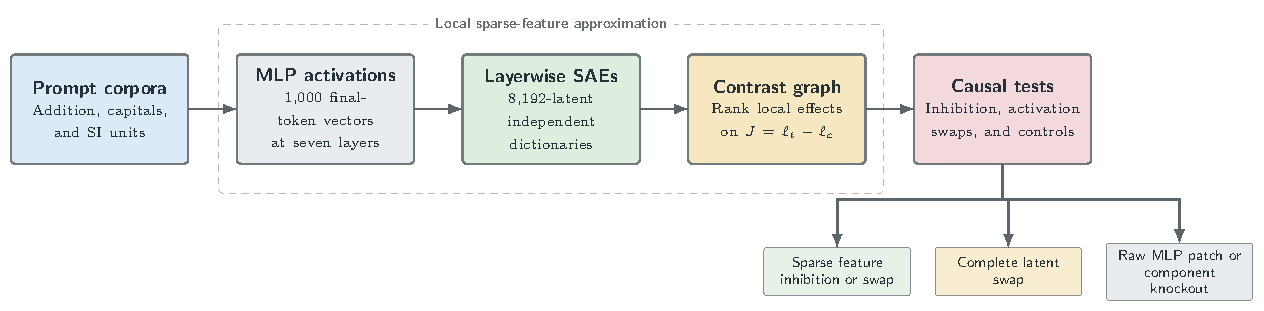
\includegraphics[width=\textwidth]{figures/fig_pipeline.pdf}
\caption{Independent small-scale reproduction pipeline, showing the stage at
which each methodological approximation is introduced.}
\label{fig:pipeline}
\end{figure}

\subsection{Causal interventions and evaluation}

Feature inhibition is error-preserving. For a selected coordinate set $S$, let
$z^{(-S)}$ equal $z$ with those coordinates set to zero. The true MLP output is
edited by only the decoded feature difference:
\begin{equation}
    x' = x+s_{\ell}W_{\mathrm d}\left(z^{(-S)}-z\right).
    \label{eq:inhibit}
\end{equation}
With $S=\varnothing$, the model is exactly unchanged. A latent swap from source
$s$ to target $t$ similarly applies
\begin{equation}
    x'_t=x_t+\alpha s_{\ell}W_{\mathrm d}(z_s-z_t),
    \label{eq:swap}
\end{equation}
where $\alpha$ is an edit strength. Sparse swaps replace only selected
coordinates; full-latent swaps use all 8,192. Raw MLP patching replaces the
selected target MLP outputs directly with source outputs and therefore bypasses
the SAE. Full knockouts set an MLP, attention or transformer-block output to zero
at specified token positions.

Interventions were initially applied at the final position and subsequently at
all aligned positions when diagnostics indicated that final-position editing was
insufficient. Token IDs and activation norms were recorded to verify that the
intended non-zero locations were modified. Effects are reported using token
probability, token logit and the contrast gap in Equation~\ref{eq:contrast}. A
change in the top-1 prediction provides direct evidence of behavioural control
but was not a necessary criterion: the clean arithmetic distribution is highly
saturated, so a substantial logit-gap change can remain informative without
altering the highest-probability token. Conversely, a prediction change under a
broad, destructive intervention does not independently identify a specific
circuit.

\section{Results}

\subsection{Baseline competence}

Table~\ref{tab:baseline} reports the retained initial baseline audit. Every
tested addition prompt was answered correctly. Performance on units and capitals
was lower, partly because these answers are multi-token and because some
templates elicited continuations such as \texttt{after} rather than an immediate
answer. Intervention effects are therefore interpreted relative to the complete
clean output distribution for the relevant prompt; low-confidence capital
examples are not considered directly comparable to high-confidence arithmetic
examples.

\begin{table}[ht]
\centering
\caption{Initial baseline audit. ``Top-$k$'' means that an acceptable answer was
found in the saved top-20/prefix-aware evaluation. These prompt counts predate
the expanded 1,000-prompt SAE corpora.}
\label{tab:baseline}
\begin{tabular}{lrrr}
\toprule
Behaviour & Prompts & Top-1 correct & In top-$k$ \\
\midrule
Addition & 200 & 200 (100.0\%) & 200 (100.0\%) \\
SI units & 200 & 134 (67.0\%) & 193 (96.5\%) \\
Capitals & 189 & 94 (49.7\%) & 158 (83.6\%) \\
\bottomrule
\end{tabular}
\end{table}

\subsection{Factual recall: SI units}

The clean force prompt predicted \texttt{new} with probability 0.8164 and logit
20.62. The matched energy prompt predicted \texttt{j} with probability 0.7969
and logit 19.88; \texttt{new} still had probability 0.0240 and logit 16.38. The
force and energy contrast graphs each contained 20 retained feature nodes per
layer. Filtering by positive node attribution selected 76 force-supporting and
97 energy-supporting features respectively.

The largest factual-recall effect was produced by the all-position full-latent
swap from force into energy. It changed the top prediction from \texttt{j} to
\texttt{new}:
\texttt{new} rose from probability 0.0240 (logit 16.38) to 0.4980 (logit 18.38),
while \texttt{j} fell from 0.7969 (19.88) to 0.2354 (17.62). The reverse
energy-to-force patch did not change the highest-probability answer, but it raised the \texttt{j} logit
from 10.06 to 14.81 and probability from below the displayed four-decimal
resolution to 0.0026, while reducing \texttt{new} probability from 0.8164 to
0.6836. Layer-wise full-latent scans placed the largest individual movements at
layers 24 and 28. For example, force-to-energy patching at layer 24 lowered the
\texttt{j} logit by 1.12 and raised \texttt{new} by 1.25.

Sparse interventions did not produce comparable transfer. Swapping all 97 positive
energy-graph features into force left the \texttt{j} logit at 10.06 and increased
\texttt{new} from 20.62 to 20.75. Swapping 76 positive force-graph features into
energy raised \texttt{new} only from logit 16.38 to 16.75 and probability 0.0240
to 0.0352; \texttt{j} remained the top token. Inhibiting the same force features
at the final position reduced \texttt{new} probability from 0.8164 to 0.8008 and
its logit by 0.24. Diagnostics confirmed that the targeted latents were active;
the small effect was therefore not attributable to the selection of inactive
coordinates.

\begin{table}[ht]
\centering
\caption{Main SI-unit swap results. Probabilities are for first-token answer
prefixes, not whole words.}
\label{tab:units}
\small
\begin{tabularx}{\textwidth}{p{0.24\textwidth}p{0.17\textwidth}XXXX}
\toprule
Target run & Intervention & $p(\texttt{j})$ & $p(\texttt{new})$ & $\ell(\texttt{j})$ & $\ell(\texttt{new})$ \\
\midrule
Energy & clean & 0.7969 & 0.0240 & 19.88 & 16.38 \\
Energy & full force latent & 0.2354 & 0.4980 & 17.62 & 18.38 \\
Energy & sparse force features & 0.8008 & 0.0352 & 19.88 & 16.75 \\
\addlinespace
Force & clean & $<0.0001$ & 0.8164 & 10.06 & 20.62 \\
Force & full energy latent & 0.0026 & 0.6836 & 14.81 & 20.38 \\
Force & sparse energy features & $<0.0001$ & 0.8242 & 10.06 & 20.75 \\
\bottomrule
\end{tabularx}
\end{table}

These results establish that the learned latent spaces contain information that
can causally alter unit-token selection, particularly in the force-to-energy
direction. They do not, however, establish a sparse-circuit reproduction: the
observed effect occurred only when the complete latent code across seven layers
and all token positions was transferred, whereas the graph-selected positive
subset was insufficient.

\begin{figure}[ht]
\centering
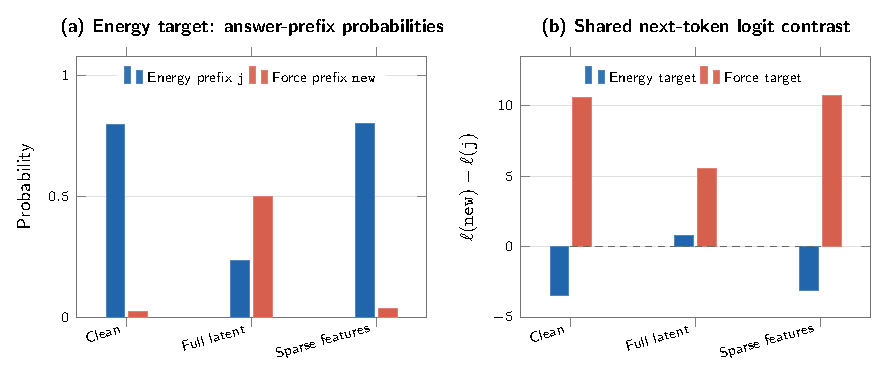
\includegraphics[width=\textwidth]{figures/fig_units_interventions.pdf}
\caption{Full-latent unit swaps transfer answer-prefix preference, whereas the
graph-selected sparse subsets do not. In panel (b), positive values of
$\ell(\texttt{new})-\ell(\texttt{j})$ favour the force prefix.}
\label{fig:units}
\end{figure}

\subsection{Addition: a carry between decimal columns}

On \code{58+83} after teacher-forcing \texttt{1}, the clean model predicted
\texttt{4} with displayed probability 1.0000 and logit 30.62. The dropped-carry
token \texttt{3} had probability 0.0008 and logit 23.50, so the clean contrast
gap was $J=7.12$. On the no-carry minimal pair \code{54+83}, the next token
\texttt{3} had displayed probability 1.0000 and logit 29.38; \texttt{4} had
probability 0.0002 and logit 20.88.

Progressive inhibition of carry-graph features produced a small, non-monotonic
response. At 10 features, the \texttt{3} logit increased by 0.12 while
\texttt{4} was unchanged. At 50 features, \texttt{4} decreased by 0.12 and
\texttt{3} increased by 0.25. With all 73 positive-attribution features,
\texttt{4} decreased by 0.38 and \texttt{3} increased by 0.12, reducing the gap
from 7.12 to 6.63. The direction is consistent with the contrast graph but the
effect is too small to establish a compact carry circuit.

Full-latent swaps were stronger. At edit strength 1, patching \code{54+83} into
\code{58+83} increased the \texttt{3} logit from 23.50 to 24.12 and probability
from 0.0008 to 0.0017; \texttt{4} remained at probability 0.9961. At strength 2,
\texttt{3} rose to probability 0.3203 and logit 27.88, while \texttt{4} fell to
0.6797 and 28.62. The contrast gap decreased to 0.74. By comparison, swapping
only the 80 positive features from the no-carry graph did not produce the
predicted directional effect: the \texttt{4} logit increased from 30.62 to 30.75
and \texttt{3} remained at 23.50.

Raw all-position MLP patching bypassed the SAE and produced a complete transfer
of the source answer at the displayed precision. Patching \code{54+83} into
\code{58+83} changed the top token from
\texttt{4} to \texttt{3}, with \texttt{3} logit 29.62 and \texttt{4} logit
21.25. The reverse patch changed the no-carry target from \texttt{3} to
\texttt{4}. These interventions establish that the selected-layer MLP outputs
contain causally sufficient information to determine the next answer digit, but
they do not identify the semantic content of that information.

The alternative-source control clarifies this ambiguity. \code{44+83=127} is
also no-carry in the ones column, but its teacher-forced next digit is
\texttt{2}, not \texttt{3}. A strength-2 full-latent patch into \code{58+83}
made \texttt{2} the top token with probability 0.6523; \texttt{3} also rose to
0.3477 and \texttt{4} fell to 0.0001. The raw MLP patch transferred \texttt{2}
with displayed probability 1.0000. The successful raw patch therefore primarily
transfers source-specific next-digit state and does not independently establish
the transfer of an abstract ``carry 1'' feature.

\begin{table}[ht]
\centering
\caption{Arithmetic interventions on the \code{58+83} tens-digit target. The
clean logits are $\ell_4=30.62$ and $\ell_3=23.50$.}
\label{tab:math}
\small
\begin{tabularx}{\textwidth}{Xrrrrl}
\toprule
Intervention & $p(4)$ & $p(3)$ & $\ell_4$ & $\ell_3$ & Interpretation \\
\midrule
Clean & 1.0000 & 0.0008 & 30.62 & 23.50 & Correct, saturated \\
73 positive features inhibited & 0.9961 & -- & 30.25 & 23.62 & Small directional shift \\
Full \code{54+83} latent, $\alpha=1$ & 0.9961 & 0.0017 & 30.50 & 24.12 & Partial shift \\
Full \code{54+83} latent, $\alpha=2$ & 0.6797 & 0.3203 & 28.62 & 27.88 & Large but non-sparse shift \\
Raw \code{54+83} MLP & 0.0002 & 1.0000 & 21.25 & 29.62 & Source digit transferred \\
Full \code{44+83} latent, $\alpha=2$ & 0.0001 & 0.3477 & 18.00 & 26.75 & Source digit 2 becomes top \\
\bottomrule
\end{tabularx}
\end{table}

The all-position MLP knockout provides complementary evidence. Zeroing the MLP
outputs at all seven selected layers reduced \texttt{4} probability to 0.6406
and logit to 27.25, while increasing \texttt{3} to probability 0.1836 and logit
26.00. However, \texttt{2} also rose to probability 0.1426 and logit 25.75.
Layer 24 alone produced the largest disruption: the model predicted \texttt{2}
with probability 1.0000, while the \texttt{4} logit fell by 10.88. Thus layer 24
is causally important for maintaining the answer, but the knockout does not show
that it represents a carry-specific variable. The result instead demonstrates a
broader dependence of digit selection on this layer's MLP output.

\begin{figure}[ht]
\centering
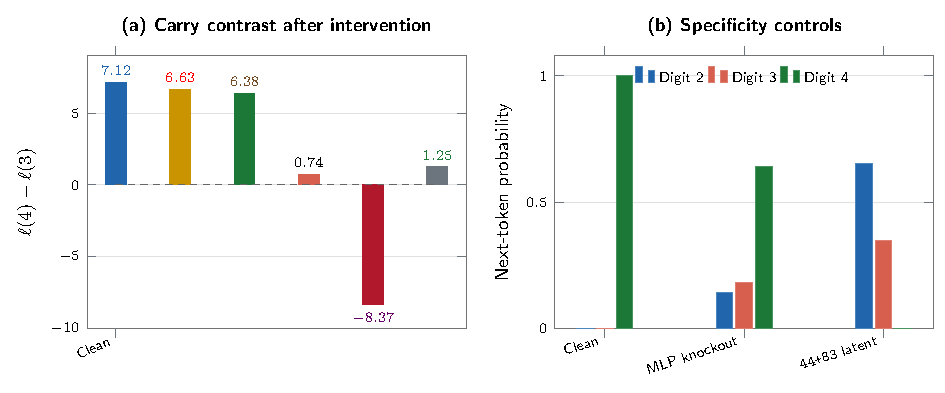
\includegraphics[width=\textwidth]{figures/fig_math_interventions.pdf}
\caption{Arithmetic interventions reveal broad causal answer state but do not
isolate a carry-specific sparse feature group.}
\label{fig:math}
\end{figure}

\subsection{Factual recall: capital cities}

The original Dallas/Oakland pair had low baseline confidence. Dallas predicted
\texttt{ Austin} with probability 0.2773, only slightly ahead of
\texttt{ Dallas} at 0.2158. For Oakland, \texttt{ Sacramento} had probability
0.2217 while \texttt{ after} was top at 0.4141. A full Oakland-to-Dallas latent
swap raised the Austin probability to 0.3281 but did not transfer Sacramento,
whose logit rose only from 2.67 to 3.97. In the reverse direction, Sacramento
rose from 0.2217 to 0.3359, but \texttt{ after} remained top at 0.3809. Sparse
swaps were smaller still.

Low baseline confidence was a plausible confound; a second pair therefore used
Zarqa to Amman and Basra to Baghdad. Clean first-token probabilities were 0.9844
for \texttt{ Am} and 0.9648 for \texttt{ Baghdad}. Higher baseline confidence did
not produce stronger causal transfer.
Patching Basra into Zarqa raised the Baghdad logit from 6.97 to 12.62, but its
probability remained 0.0002 and \texttt{ Am} remained top at 0.9805. The reverse
patch reduced Baghdad probability from 0.9648 to 0.8711 and raised the Amman
prefix from 0.0001 to 0.0002. Graph-selected sparse swaps caused negligible
changes in both directions. Capital recall therefore constitutes a weak or
negative reproduction whose outcome cannot be attributed solely to low prompt
confidence.

\begin{figure}[ht]
\centering
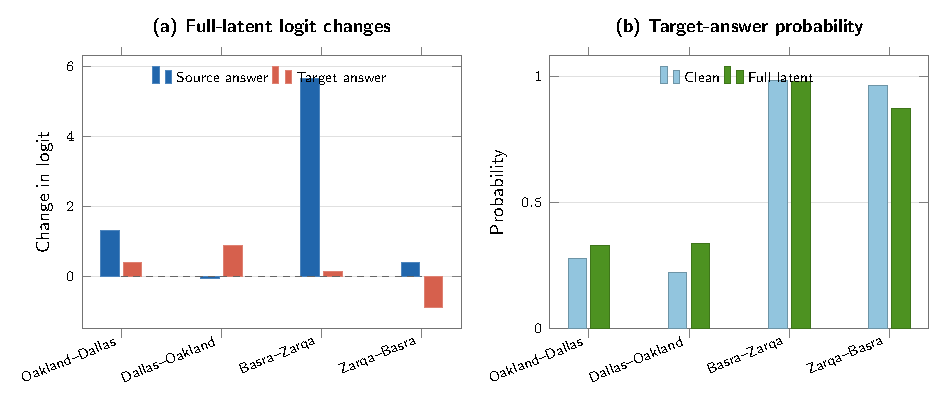
\includegraphics[width=\textwidth]{figures/fig_capitals_interventions.pdf}
\caption{Capital-city full-latent interventions. Panel (a) reports changes in
the source- and target-answer logits; panel (b) compares the target-answer
probability before and after intervention. The high-confidence Basra--Zarqa
control reduces one potential confound but does not yield clear answer transfer.}
\label{fig:capitals}
\end{figure}

\section{Discussion}

\subsection{Extent of reproduction}

The first research question yields a qualified negative result. Aggregate
inhibition of graph-selected features occasionally moved the pre-specified
contrast in the expected direction, most clearly in the arithmetic scan.
However, no graph-selected sparse swap produced a clear transfer of a tested
answer. The evidence is therefore insufficient to classify the result as a
sparse-circuit reproduction.

The evidence concerning the second research question is more affirmative. Full
latent codes and raw MLP outputs contain causally effective information. The
force-to-energy unit patch changes the most probable answer prefix, the stronger
no-carry arithmetic latent patch nearly equalises the correct and dropped-carry
digits, and raw MLP patches transfer source digits in both directions. These
controls distinguish two possible failure modes: transferable internal state is
present in the model, but the selected sparse coordinates do not constitute a
compact causal basis for that state.

The alternative arithmetic source substantially constrains interpretation of
the apparent transfer. In its absence, the
\code{54+83}\,$\rightarrow$\,\code{58+83} prediction change could be interpreted
as transfer of a no-carry mechanism. The transfer of \texttt{2} from
\code{44+83} instead supports the narrower conclusion that broad patches
transfer source-specific answer state. Evidence for a carry variable would
require generalisation across multiple source--target pairs in which carry
status and output digit are independently varied.

The findings reproduce the methodological structure of the target study but are
substantially weaker at the level of sparse causal control. The study established
the behaviour, selected a decisive logit contrast, constructed a pruned feature
graph, derived interventions and evaluated them in the underlying model. It did
not recover a compact sparse-feature mechanism. This outcome is consistent with
the target study's report that cross-layer transcoders outperform per-layer
alternatives and that mechanistic faithfulness requires empirical evaluation
rather than assumption \cite{ameisen2025circuit}.

\subsection{Divergence between reconstruction and sparse causal control}

Several methodological differences provide testable explanations for the gap
between reconstruction performance and sparse causal control. These explanations
do not require an unsupported assumption that the discrepancy arises solely
from model-specific properties of Qwen.

\paragraph{The implemented $\ell_1$ objective is scale-degenerate.}
Equation~\ref{eq:sae-loss} penalises latent magnitude, but the decoder columns
are not constrained to unit norm. For any $c>0$, consider the rescaling
\begin{equation}
    W_{\mathrm e}'=cW_{\mathrm e},\qquad b_{\mathrm e}'=cb_{\mathrm e},
    \qquad W_{\mathrm d}'=\frac{1}{c}W_{\mathrm d}.
\end{equation}
Positive homogeneity of ReLU gives $z'=cz$, while
$W_{\mathrm d}'z'=W_{\mathrm d}z$. Reconstruction is unchanged but the $\ell_1$ term
is multiplied by $c$ and can, in principle, be made arbitrarily small. This
property does not demonstrate that optimisation fully exploited the degeneracy,
and ReLU can still produce exact zeros. It does establish that the raw $\ell_1$ term
is not an invariant measure of sparsity and that $\lambda$ alone cannot guarantee
a sparse code. Decoder normalisation, an $\ell_0$-oriented nonlinearity such as
JumpReLU, or a scale-aware penalty would remove or reduce this ambiguity. The
target CLT used a decoder-norm-aware Tanh penalty rather than the present raw $\ell_1$ term
\cite{ameisen2025circuit}.

\paragraph{The dictionaries are underconstrained by the activation sample.}
Each per-layer SAE has approximately 42 million trainable parameters but only
800 training vectors. The 1,000 prompts are also highly templated: units span
five quantities and ten repeated syntactic forms. Low validation reconstruction
loss on the same prompt distribution therefore does not establish feature
uniqueness, monosemanticity or causal generalisation. Final $\ell_0$ firing-rate,
dead-feature and feature-consistency diagnostics were not retained.
Consequently, no quantitative claim about achieved sparsity is made.

\paragraph{Training and intervention supports do not always match.}
SAEs were trained only on final-token MLP outputs. All-position latent
interventions then encoded every prompt position, including words and digits,
with those final-position dictionaries. This is out of distribution by
construction. The mismatch is most pronounced in arithmetic: training prompts ended
at \texttt{Answer:}, whereas the carry graph and swaps operate after a
teacher-forced \texttt{1}. The exact force prompt also appears in the generated
unit corpus, whereas the synthetically modified energy minimal pair does not; the
principal unit result therefore does not constitute a strictly held-out
generalisation test. These limitations do not invalidate the observed
forward-pass changes, but they restrict the extent to which those changes support
claims about stable, distribution-independent features.

\paragraph{The graph is a smaller local approximation.}
Only final-position SAE features are nodes. Attention and normalisation are not
frozen, and reconstruction discrepancies are not represented as explicit error
nodes. The straight-through splice guarantees the clean value, but its gradients
remain a first-order local approximation through the original nonlinear model.
The graph can consequently rank locally sensitive coordinates without providing
the same replacement-model semantics as Anthropic's CLT graph. Positive node
attribution is also not guaranteed to imply a large finite ablation effect when
features interact nonlinearly.

\paragraph{Saturation and intervention specificity matter.}
The clean arithmetic gap of 7.12 logits leaves little probability mass on
\texttt{3}; small but real logit changes are visually compressed. Increasing
edit strength exposes a larger effect, but also moves farther from the local
regime in which gradient attribution is most defensible. Component knockout
presents a different inferential limitation: it establishes causal dependence
but is too destructive to provide mechanistic specificity. The increase in both
\texttt{2} and \texttt{3}, together with the layer-24 change to \texttt{2},
demonstrates that a change in the highest-probability token does not by itself
identify a carry circuit.

\subsection{Threats to validity}

The study is exploratory and uses selected prompts rather than a registered
large-sample intervention benchmark. The forward passes are deterministic, but
only one SAE seed was used, so feature identities and sparse effects have no
between-seed stability estimate. Prompt corpora supply train and validation
splits for reconstruction, but the intervention prompts were not consistently
reserved as an independent test set. Aggregate baseline outputs were retained
from an earlier, smaller dataset version, while final SAE training used the
expanded corpora. These baseline percentages should therefore be treated as
competence checks, not confidence intervals for final test accuracy.

Tokenisation also constrains interpretation. Unit and capital answers are often
multi-token, so the experiments intervene on first-token prefixes rather than
complete answer strings. Arithmetic teacher forcing isolates a decimal position
but changes the activation context relative to SAE training. Finally, bfloat16
execution and single-run reporting make changes of roughly 0.1 logits weak
evidence unless they form a coherent pattern or are supported by stronger
controls.

A post-experiment code audit identified one reporting defect: the saved raw-MLP
layer-scan path patched every requested layer in each nominal single-layer row.
Consequently, the repeated per-layer raw-scan rows are excluded from the present
analysis. The aggregate raw MLP patches, full knockouts and SAE layer scans use
separate execution paths and are unaffected. The hook-selection error has been
corrected in the repository. Exclusion of the affected rows prevents an invalid
layer-localisation inference.

\subsection{Prioritised future work}

The highest-priority extension is to align the random variables represented in
SAE training with those modified during causal evaluation. Increasing the number
of training epochs without resolving this mismatch would provide limited
additional evidence.

\begin{enumerate}
    \item Capture activations at all token positions, or at a pre-specified set of
    intervention positions, and include teacher-forced partial answers in the
    arithmetic SAE corpus.
    \item Retrain with decoder-column normalisation or a gated/JumpReLU objective;
    report $\ell_0$ firing counts, dead-feature rates, reconstruction variance and
    clean-model recovery before interpreting features.
    \item Build a held-out factorial carry benchmark. Carry status, source next
    digit and target next digit should vary independently across many matched
    pairs. Rank features by their marginal effect on
    $\ell(\text{correct})-\ell(\text{dropped carry})$ across examples rather than
    on a single prompt.
    \item Repeat SAE training across seeds and test whether feature groups, not
    exact feature indices, reproduce their causal effects.
    \item Subject to available computational resources, replace independent output SAEs with per-layer
    transcoders or a small cross-layer transcoder and add explicit residual/error
    nodes. Compare model-level recovery and perturbation faithfulness at matched
    feature budgets.
    \item Extend the graph to attention or residual-stream features. The weak
    sparse MLP result does not establish that the missing mechanism is absent;
    it may be represented in attention-mediated state or SAE reconstruction
    error.
\end{enumerate}

These steps would discriminate among the explanations advanced here. In
particular, improved sparse effects after position-matched training would support
distribution mismatch as the main cause; persistence of broad raw-patch effects
without stable sparse features would support a genuinely distributed or
interaction-dependent representation.

\section{Conclusion}

The present study independently implemented a small-scale mechanistic-
interpretability pipeline for an open-weight language model. The pipeline
generated and audited behavioural prompts, captured selected MLP activations,
trained per-layer SAEs, constructed contrast attribution graphs, and evaluated
them using feature inhibition, latent swaps and activation-level controls. The
principal positive finding is a hierarchy of causal effects rather than an
isolated feature: raw MLP state can transfer an arithmetic answer; complete SAE
latent state can substantially alter arithmetic and unit predictions; and sparse
graph-selected subsets generally cannot. Capital recall provides a negative
result even after baseline confidence was increased.

The evidence therefore supports transfer of the experimental methodology more
strongly than recovery of a sparse circuit. Under the lightweight Qwen
implementation, attribution graphs generate testable causal hypotheses, but
their highest-attribution SAE nodes do not consistently constitute a compact,
faithful mechanism. The mathematical and methodological analysis identifies
four specific limitations---scale-degenerate sparsity, limited activation
support, positional distribution mismatch and a less expressive local
replacement model---that yield testable explanations for the partial
reproduction. The study thereby establishes both whether the target effects were
observed and the conditions under which the corresponding mechanistic inferences
are warranted.

\begin{thebibliography}{9}

\bibitem{lindsey2025biology}
J. Lindsey, W. Gurnee, E. Ameisen, et al.,
``On the Biology of a Large Language Model,''
\emph{Transformer Circuits Thread}, 2025.
\url{https://transformer-circuits.pub/2025/attribution-graphs/biology.html}

\bibitem{ameisen2025circuit}
E. Ameisen, J. Lindsey, A. Pearce, et al.,
``Circuit Tracing: Revealing Computational Graphs in Language Models,''
\emph{Transformer Circuits Thread}, 2025.
\url{https://transformer-circuits.pub/2025/attribution-graphs/methods.html}

\bibitem{cunningham2023sae}
H. Cunningham, A. Ewart, L. Riggs, R. Huben, and L. Sharkey,
``Sparse Autoencoders Find Highly Interpretable Features in Language Models,''
\emph{arXiv preprint arXiv:2309.08600}, 2023.
\url{https://arxiv.org/abs/2309.08600}

\bibitem{bricken2023monosemanticity}
T. Bricken, A. Templeton, J. Batson, et al.,
``Towards Monosemanticity: Decomposing Language Models With Dictionary Learning,''
\emph{Transformer Circuits Thread}, 2023.
\url{https://transformer-circuits.pub/2023/monosemantic-features/index.html}

\bibitem{elhage2022superposition}
N. Elhage et al.,
``Toy Models of Superposition,''
\emph{Transformer Circuits Thread}, 2022.
\url{https://transformer-circuits.pub/2022/toy_model/index.html}

\bibitem{yang2025qwen3}
A. Yang, A. Li, B. Yang, et al.,
``Qwen3 Technical Report,''
\emph{arXiv preprint arXiv:2505.09388}, 2025.
\url{https://arxiv.org/abs/2505.09388}

\bibitem{qwenmodelcard}
Qwen Team,
``Qwen3-4B-Instruct-2507 Model Card,'' 2025.
\url{https://huggingface.co/Qwen/Qwen3-4B-Instruct-2507}

\end{thebibliography}

%TC:ignore
\section*{Declaration of use of autogeneration tools}
\addcontentsline{toc}{section}{Declaration of use of autogeneration tools}

Generative AI tools, including OpenAI Codex, were used during software
development to assist with code review, debugging, experimental documentation,
and the structuring and drafting of this report. GPU experiments were executed by
the candidate. The candidate remains responsible for checking the final
analysis, numerical claims, citations, wording and conclusions. This declaration
describes the use of these tools in the preparation of the submitted work.
% Verify this declaration against any course-prescribed wording before submission.
%TC:endignore

\end{document}
